\documentclass{article}
\usepackage{KJN}
\usepackage{a4wide,changebar}
\usepackage[numbered,framed]{mcode}

\title{Introduction to Vision and Robotics: Assignment 1}
\author{Chris Swetenham: Student Num, Daniel Mankowitz: S1128165}
\date{3/11/2011}

\begin{document}
\maketitle

\section{Introduction}
\label{sec:introduction}
%An overview of the main ideas used in the approach


\section{Methods}
\label{sec:methods}
%Describe the vision techniques used

%Detail how these ideas were implemented

%Describe the structure of the code

%How each part is meant to work

%Justify design decisions where appropriate

\subsection{Initial Processing}
\label{sec:processing}

\begin{figure}[htbp!] 
  \centering
    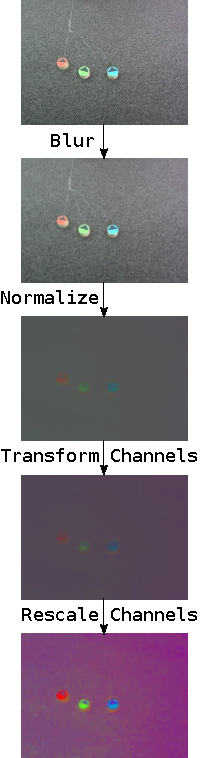
\includegraphics[width=0.3\textwidth]{../Drawings/processing.pdf}
    \caption{Image Processing Pipeline}
    \label{fig:processing}
\end{figure}

The first part of the algorithm, summarised in Figure~\ref{fig:processing}, processes each image to minimise variations both between datasets and across each image. First, the image is blurred using a gaussian kernel of width 5; this removes some of the noise in the image which would cause trouble in later stages. Next, the rgb value of each pixel is normalized; this corrects for variations in illumination across the image. At this stage, the green channel is modified by subtracting 0.2 times the blue channel. This is because the colours of the cars are not a pure value in a single channel; in particular, the blue car shows up brightly on the green channel. This simple operation is equivalent to finding a new "green car channel" attuned particularly to the green car. If the cars were other colours, such as cyan, magenta and yellow, we could have constructed dedicated channels for each car; but in this case a simple tweak to the green channel was enough to disambiguate the cars. Finally, each colour channel is scaled so that the minimum and maximum values present in the channel map to 0 and 1. This helps the thresholding after detection.

The detection algorithm a single image, and identifies the most likely location of the red, green and blue cars.
Once these steps have been performed, the algorithm estimates the location of each car in the image using the corresponding colour channel. For the red car for instance, it looks at the red channel, and computes the maximal value for each row, and for each column. It convolves each of these to reduce noise, and finds the maximum along the rows and maximum along the columns. The corresponding x and y coordinate are the identified centre of the car. The algorithm takes a 120x120 bounding box around the centre, and passes the image to the next stage for finer-grained processing.
(Is this equivalent to just blurring the image and finding the x, y coord of the maximum, then thresholding at 75\% of that value?)

\subsection{Linking Algorithm}
\label{sec:linking}
The linking algorithm is used to link together detections of a single robot in consecutive frames. Since the images provided in the dataset are RGB, the linking algorithm has been implemented to run on each of the three colour channels respectively. 

The algorithm is shown in \figref{fig:link}. Initially, the image on the $k^{th}$ iteration will have been split into three colour channels of red, green and blue respectively. Each colour channel is represented as a separate image. The robots in each colour channel will have been identified and their optimum bounding boxes need to be calculated. These images are fed into the linking algorithm. 


\begin{figure}[h!] 
  \centering
    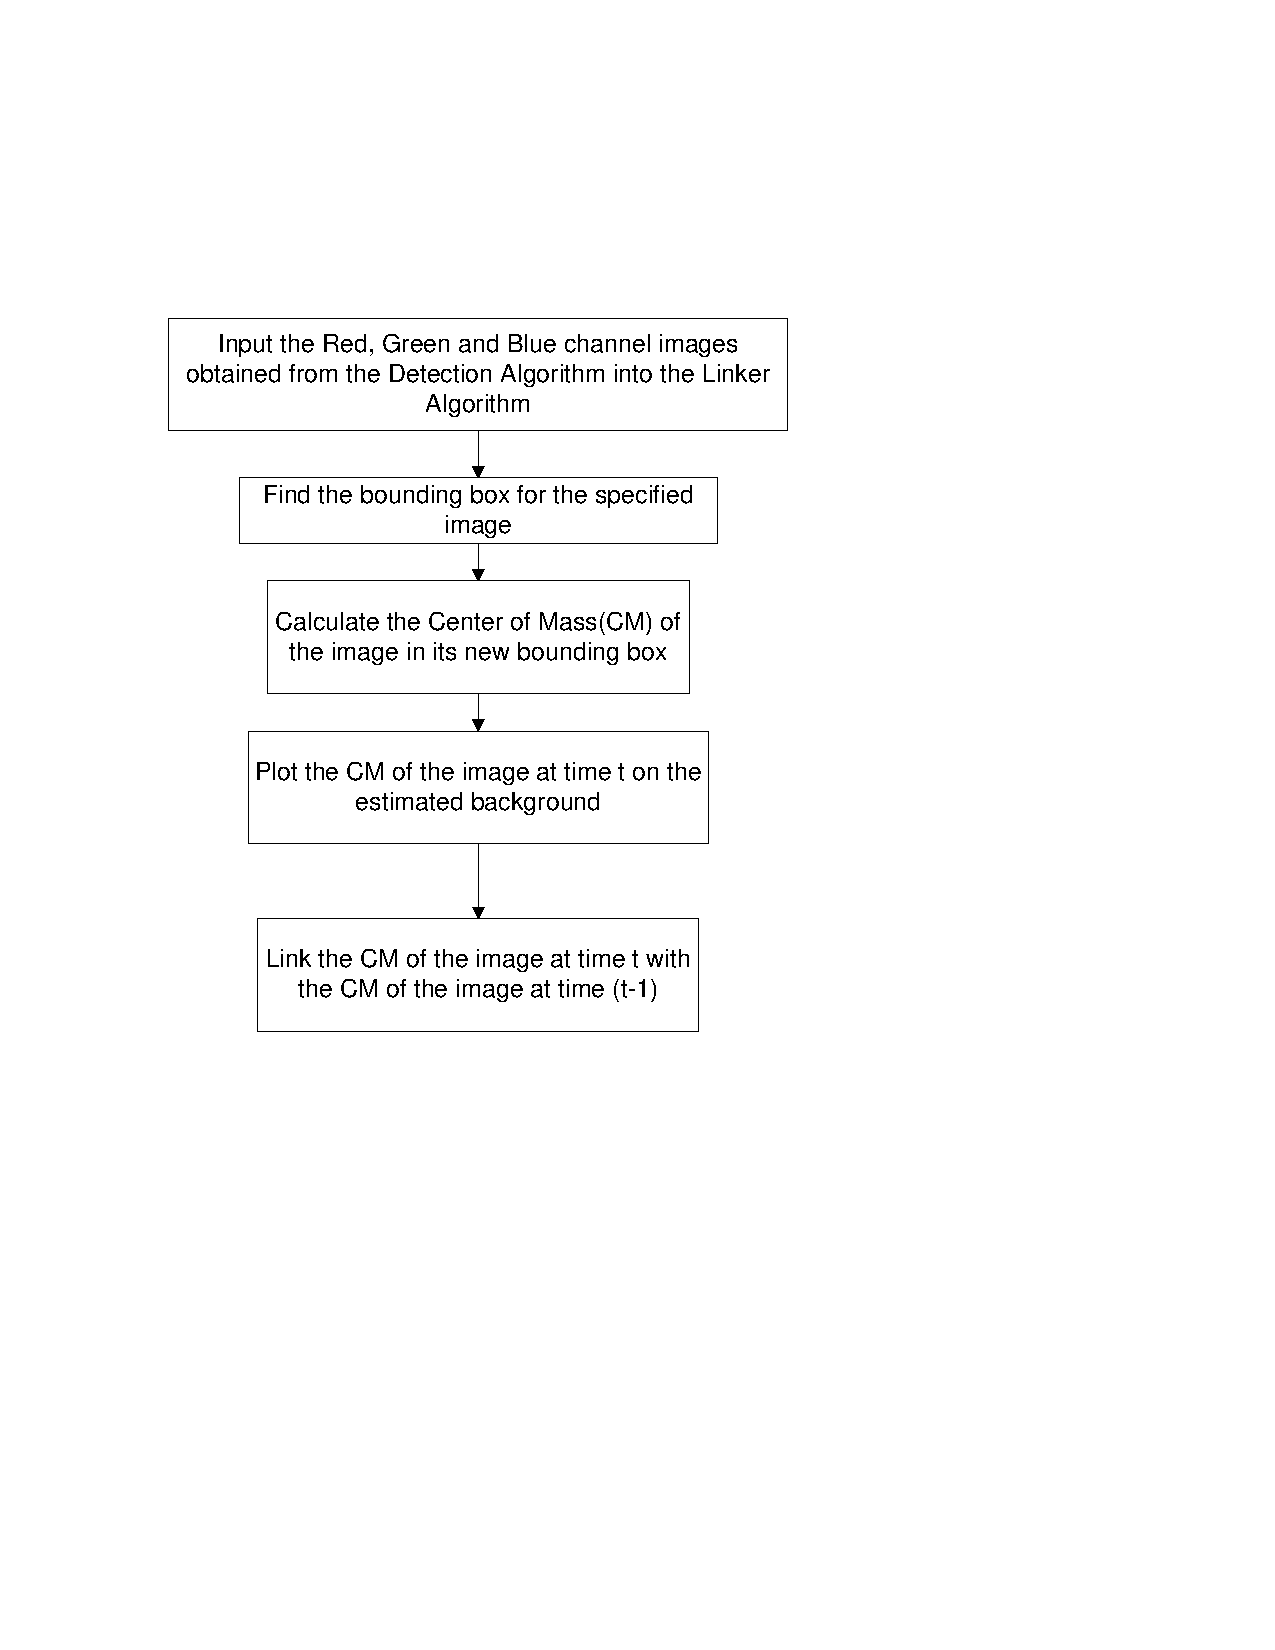
\includegraphics[width=0.5\textwidth]{../Drawings/linkingAlgorithm.pdf}
    \caption{The algorithm developed to link detections of the robot in consecutive frames}
    \label{fig:link}
\end{figure}


Once the images containing the robots have been received, a bounding box for each robot is calculated as well as the box's corresponding centroid. This is achieved in code using the `calcBoundingBox' function. This function has been developed according to \figref{fig:bounding}. Each image is labelled using the `mybwlabel' function. This will identify all of the objects in the image. The object with the largest area (I.e. the robot) will then be surrounded by its corresponding bounding box. The centroid of this bounding box is then calculated. This is performed on each of the three images corresponding to their repective colour channels.

\begin{figure}[h!] 
  \centering
    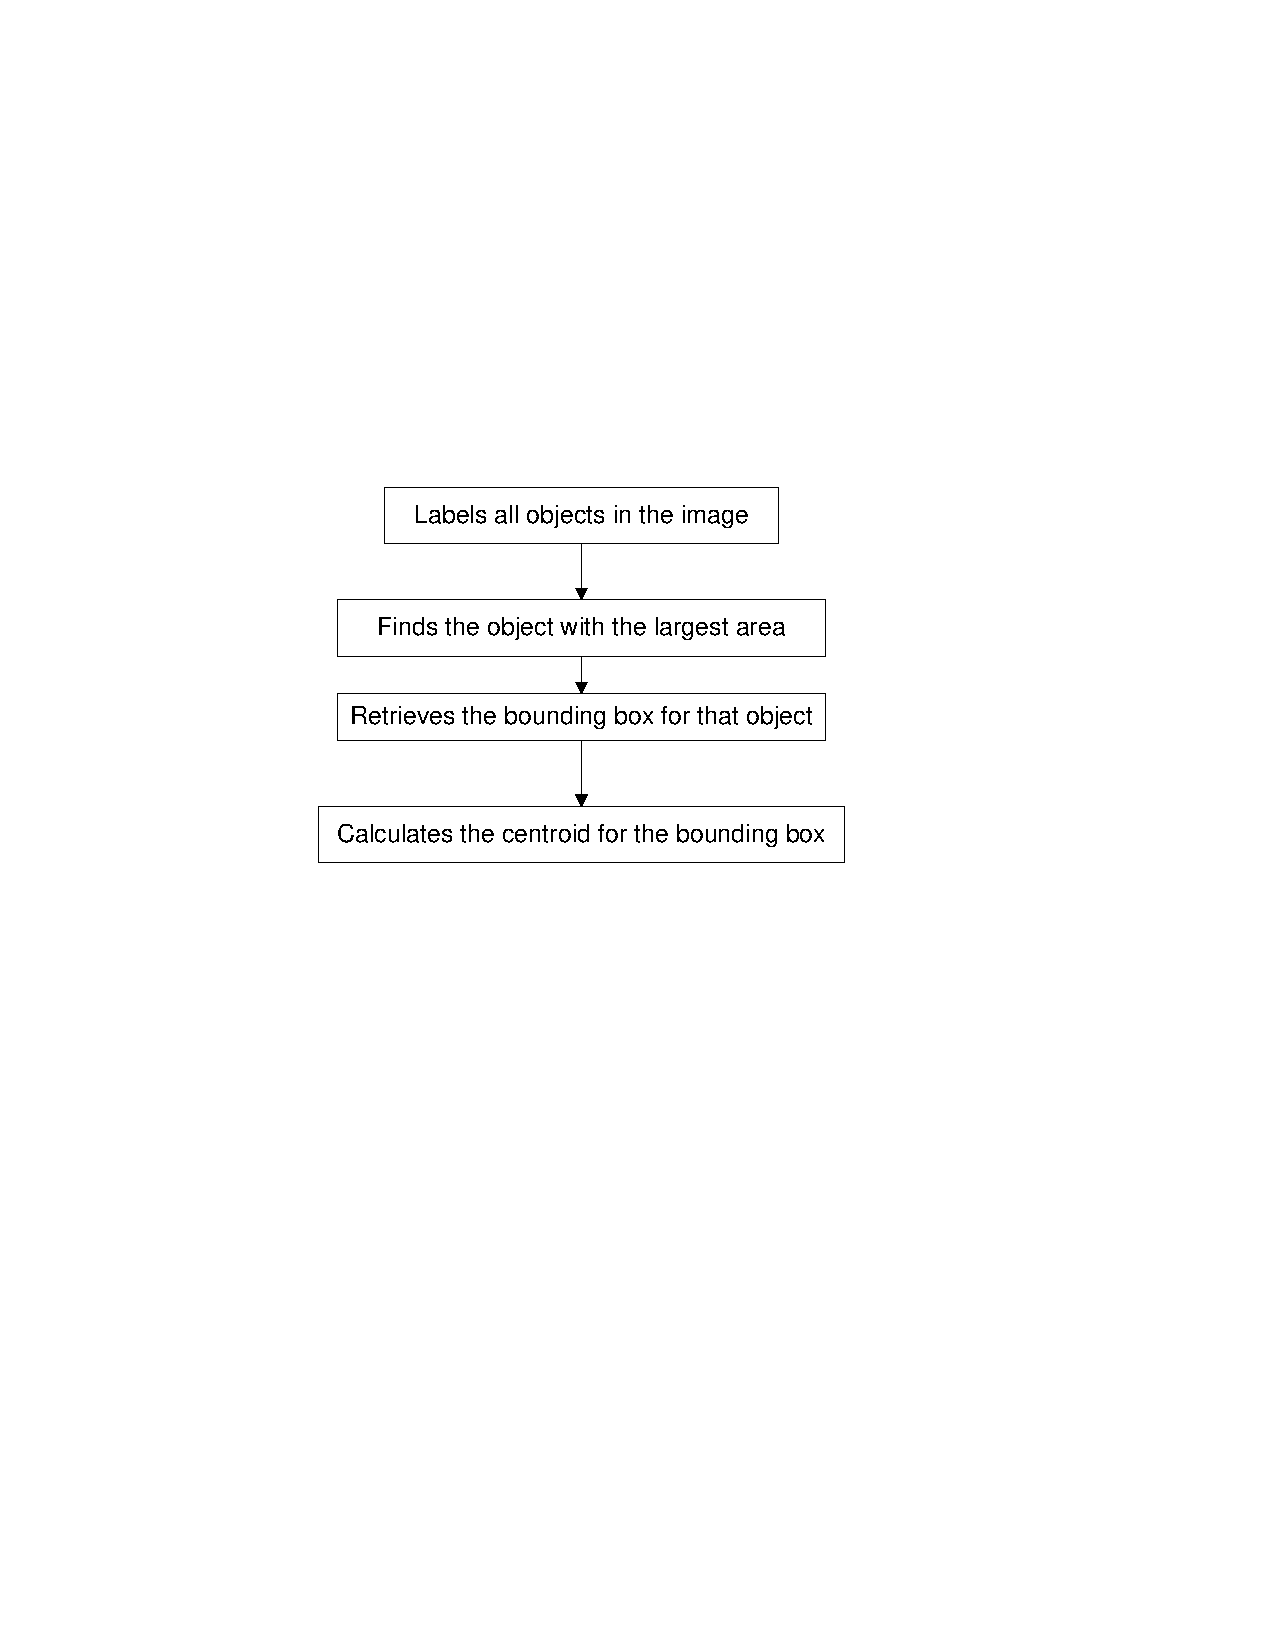
\includegraphics[width=0.5\textwidth]{../Drawings/boundingbox.pdf}
    \caption{The bounding box calculation for each robot }
    \label{fig:bounding}
\end{figure}

Once a bounding box for the robot has been determined, the center of mass of the robot needs to be calculated. This is achieved by utilising the `calcBoundingBoxCM' function.

This algorithm makes use of two important equations shown in \eqnref{eqn:area} and \eqnref{eqn:cm} respectively.

\begin{equation}
A = \Sigma_{r}\Sigma_{c}P_{rc}
\label{eqn:area}
\end{equation}

\begin{equation}
(\widehat{r}, \widehat{c}) = (\frac{1}{A}\Sigma_{r}\Sigma_{c}r P_{rc}, \frac{1}{A}\Sigma_{r}\Sigma_{c}c P_{rc})
\label{eqn:cm}
\end{equation}

\subsection{Background Estimation}
\label{sec:back}
Estimation of the background image required the implementation of a variety of different image processing techniques. This is because the datasets provided presented a number of challenges. One such challenge was that of removing robots that were stationary for a significant portion of a frame sequence. This prevented the simple implementation of a median filter to calculate the background image. This is due to the fact that objects that are stationary for a large subset of the frames will be incorporated into the median and subsequently into the background image.\\

Therefore, in order to solve this problem, an algorithm has been developed to calculate the background image, regardless of stationary robots being in large subsets of the frame sequence. \\

The background estimation algorithm consists of three main functional blocks. These blocks are \textit{Channel Processing}, \textit{Region Erasing and Filling} and \textit{Median Filtering} respectively. The \textit{Channel Processing} block receives an image frame and processes the image. This includes blurring, normalising, separating the image into its three channels, subtracting the blue channel from the green channel and renormalising the image. This creates an image that is ready for \textit{Region Erasing and Filling}. In order to implement this functional block, the image channels for the current frame are input into a function called \textit{eraseRegion}. A code snippet of the function is shown below.

\lstinputlisting{eraseRegion.m}

This function calculates the average value of the pixels found at the corner vertices of the bounding boxes surrounding each robot as shown in \figref{fig:vertices}. The corner pixels are averaged across all three colour channels and are stored in the variable \textit{Avg}. All of the pixels in the region containing the robot are then filled with this new average value to produce the image shown in \figref{fig:vertices}. This is applied to each of the robots in the image. 

\begin{figure}[h!]
	\centering
		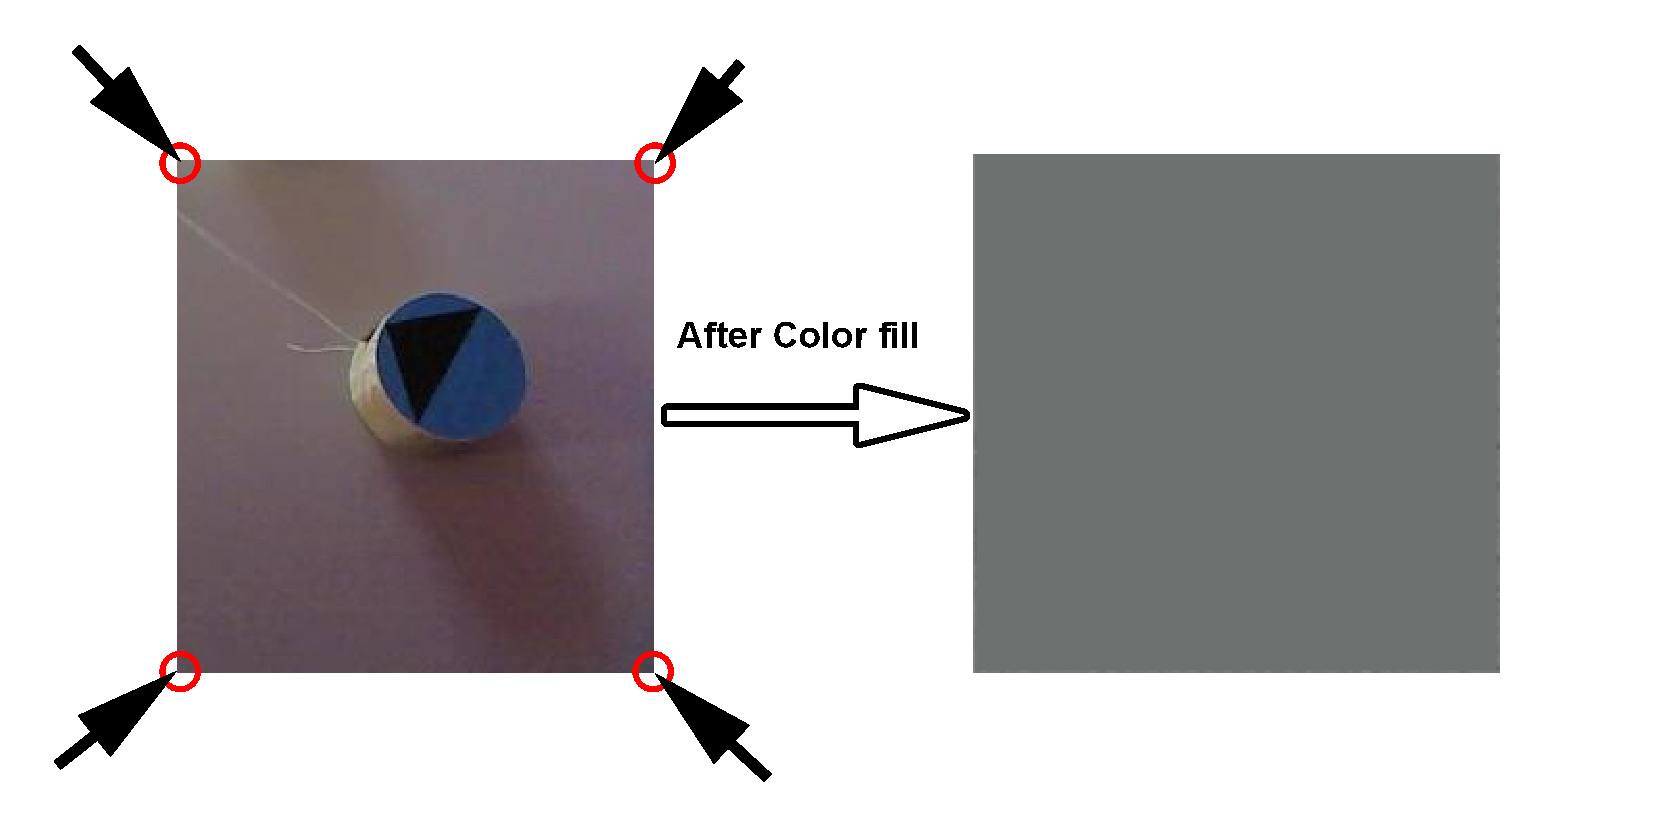
\includegraphics[width=0.8\textwidth]{../Drawings/backgroundErasingMain.pdf}
	\caption{The corner pixel intensities are averaged and are then used to fill the region of the image containing the robot}
	\label{fig:vertices}
\end{figure}

The \textit{Region Erasing and Filling} functional block is implemented on the three image frames that are used for background estimation. The reason three image frames have been chosen is because this is the minimum number of frames required to effectively use a median filter which is utilised in the \textit{Median Filtering} functional block. In addition to this, using a small number of frames to compute the median minimises the algorithm's processing time. The median of the three images is subsequently computed to produce an estimation of the background image.

\section{Results}
\label{sec:results}
%Test data
\subsection{Robot Detection}
\label{sec:detect}
An example of an incorrect detection of a robot due to the robot leaving the image frame.

\begin{figure}[h!]
\begin{minipage}[b]{0.5\linewidth}
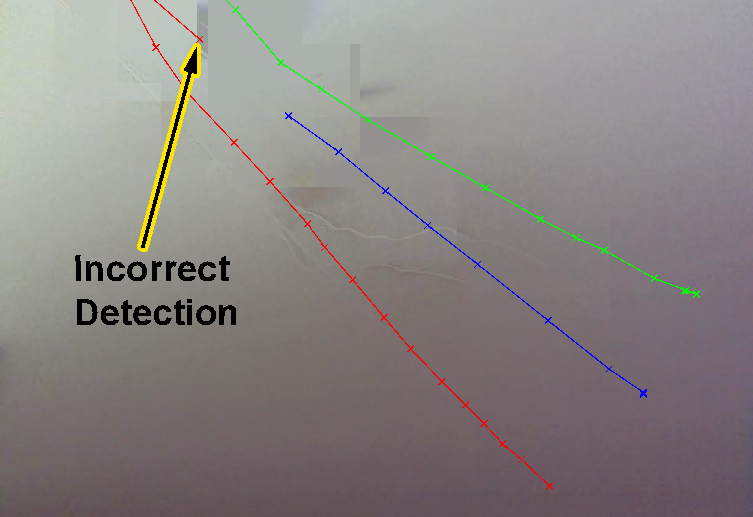
\includegraphics[scale=0.5]{../Drawings/incorrectdetBackdata1.pdf}
\caption{An incorrect detection of a robot}
\label{fig:InDetectData2}
\end{minipage}
\hspace{0.5cm}
\begin{minipage}[b]{0.5\linewidth}
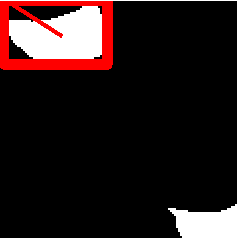
\includegraphics[scale=0.8]{../Drawings/incorrectdetrobotdata1.pdf}
\caption{The incorrect detection of the red robot as shown in the red channel thresholded image}
\label{fig:redInDetect}
\end{minipage}
\end{figure}

An example of an incorrect detection of a robot due to a region of highly saturated pixels that have a similar colour to that of the robot.

\begin{figure}[h!]
\begin{minipage}[b]{0.5\linewidth}
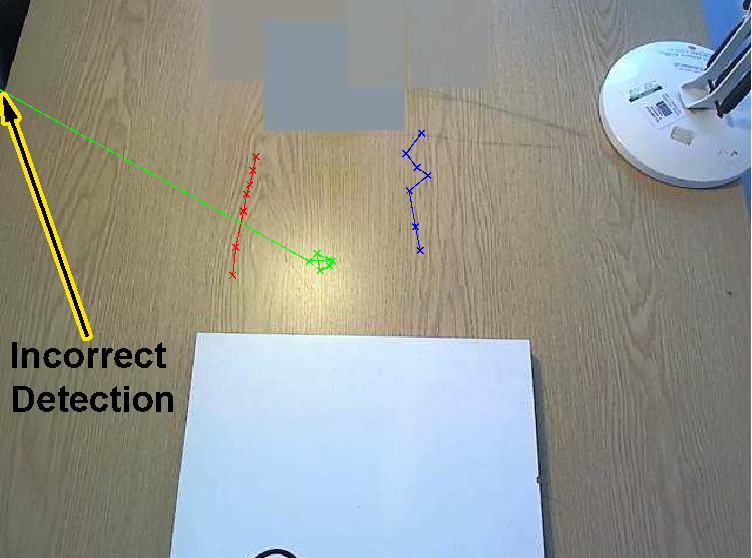
\includegraphics[scale=0.5]{../Drawings/incorrectdetBackdata7.pdf}
\caption{An incorrect detection of the green robot}
\label{fig:InDetectData7}
\end{minipage}
\hspace{0.5cm}
\begin{minipage}[b]{0.5\linewidth}
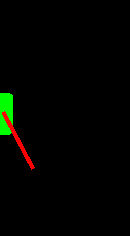
\includegraphics[scale=0.8]{../Drawings/incorrectdetrobotdata7.pdf}
\caption{The incorrect detection of the green robot due to a small region of highly saturated pixels}
\label{fig:greenInDetect}
\end{minipage}
\end{figure}


\subsection{Robot Orientation}
\label{sec:orient}
An example of incorrect and missed orientation in an image frame.

\begin{figure}[h!]
	\centering
		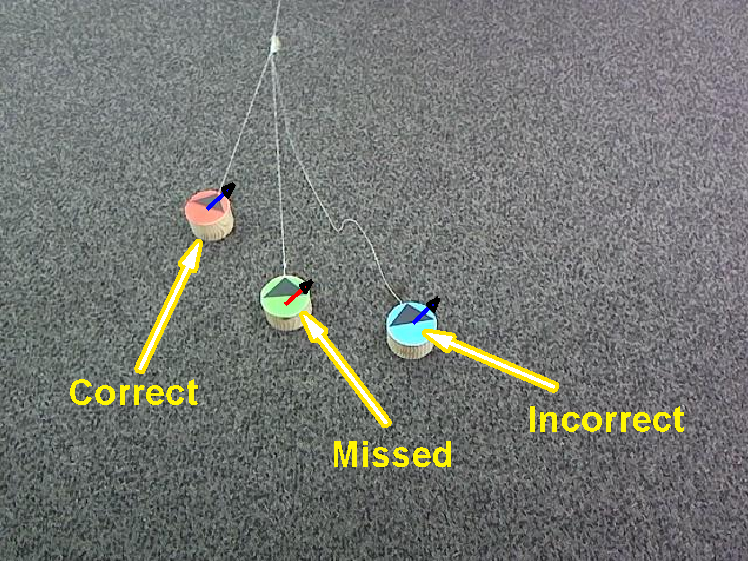
\includegraphics[width=0.6\textwidth]{../Drawings/missedandIncorrectDetData2Ready.pdf}
	\caption{Examples of incorrect and missed detections of invalid arrow orientations}
	\label{fig:indetect}
\end{figure}


\subsection{Background Images}
\label{sec:back}
An example of background images produced using the Background Estimation Algorithm detailed in \secref{sec:back}.

\begin{figure}[h!]
\begin{minipage}[b]{0.5\linewidth}
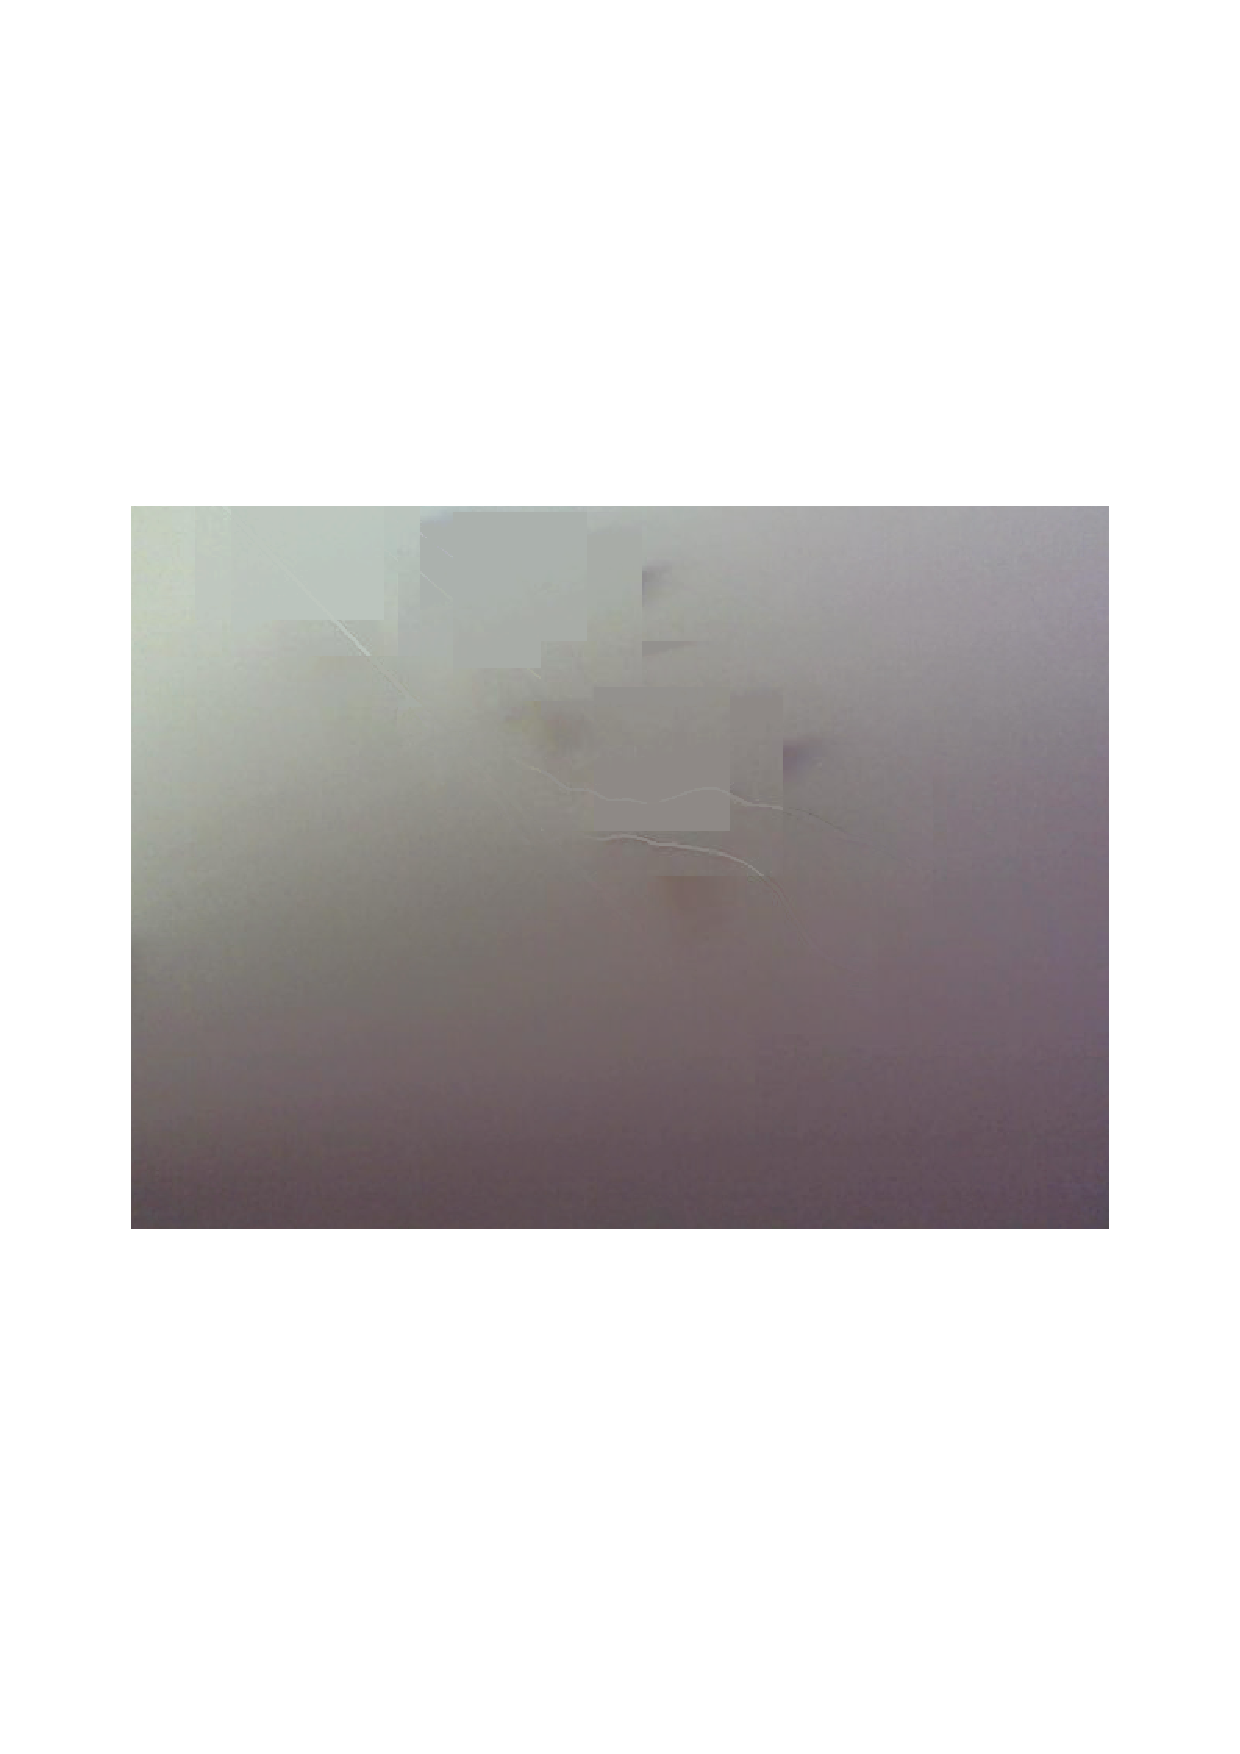
\includegraphics[scale=0.4]{../Drawings/backdata1.pdf}
\caption{The estimated background image of the first dataset provided for image processing}
\label{fig:backdata1}
\end{minipage}
\hspace{0.5cm}
\begin{minipage}[b]{0.5\linewidth}
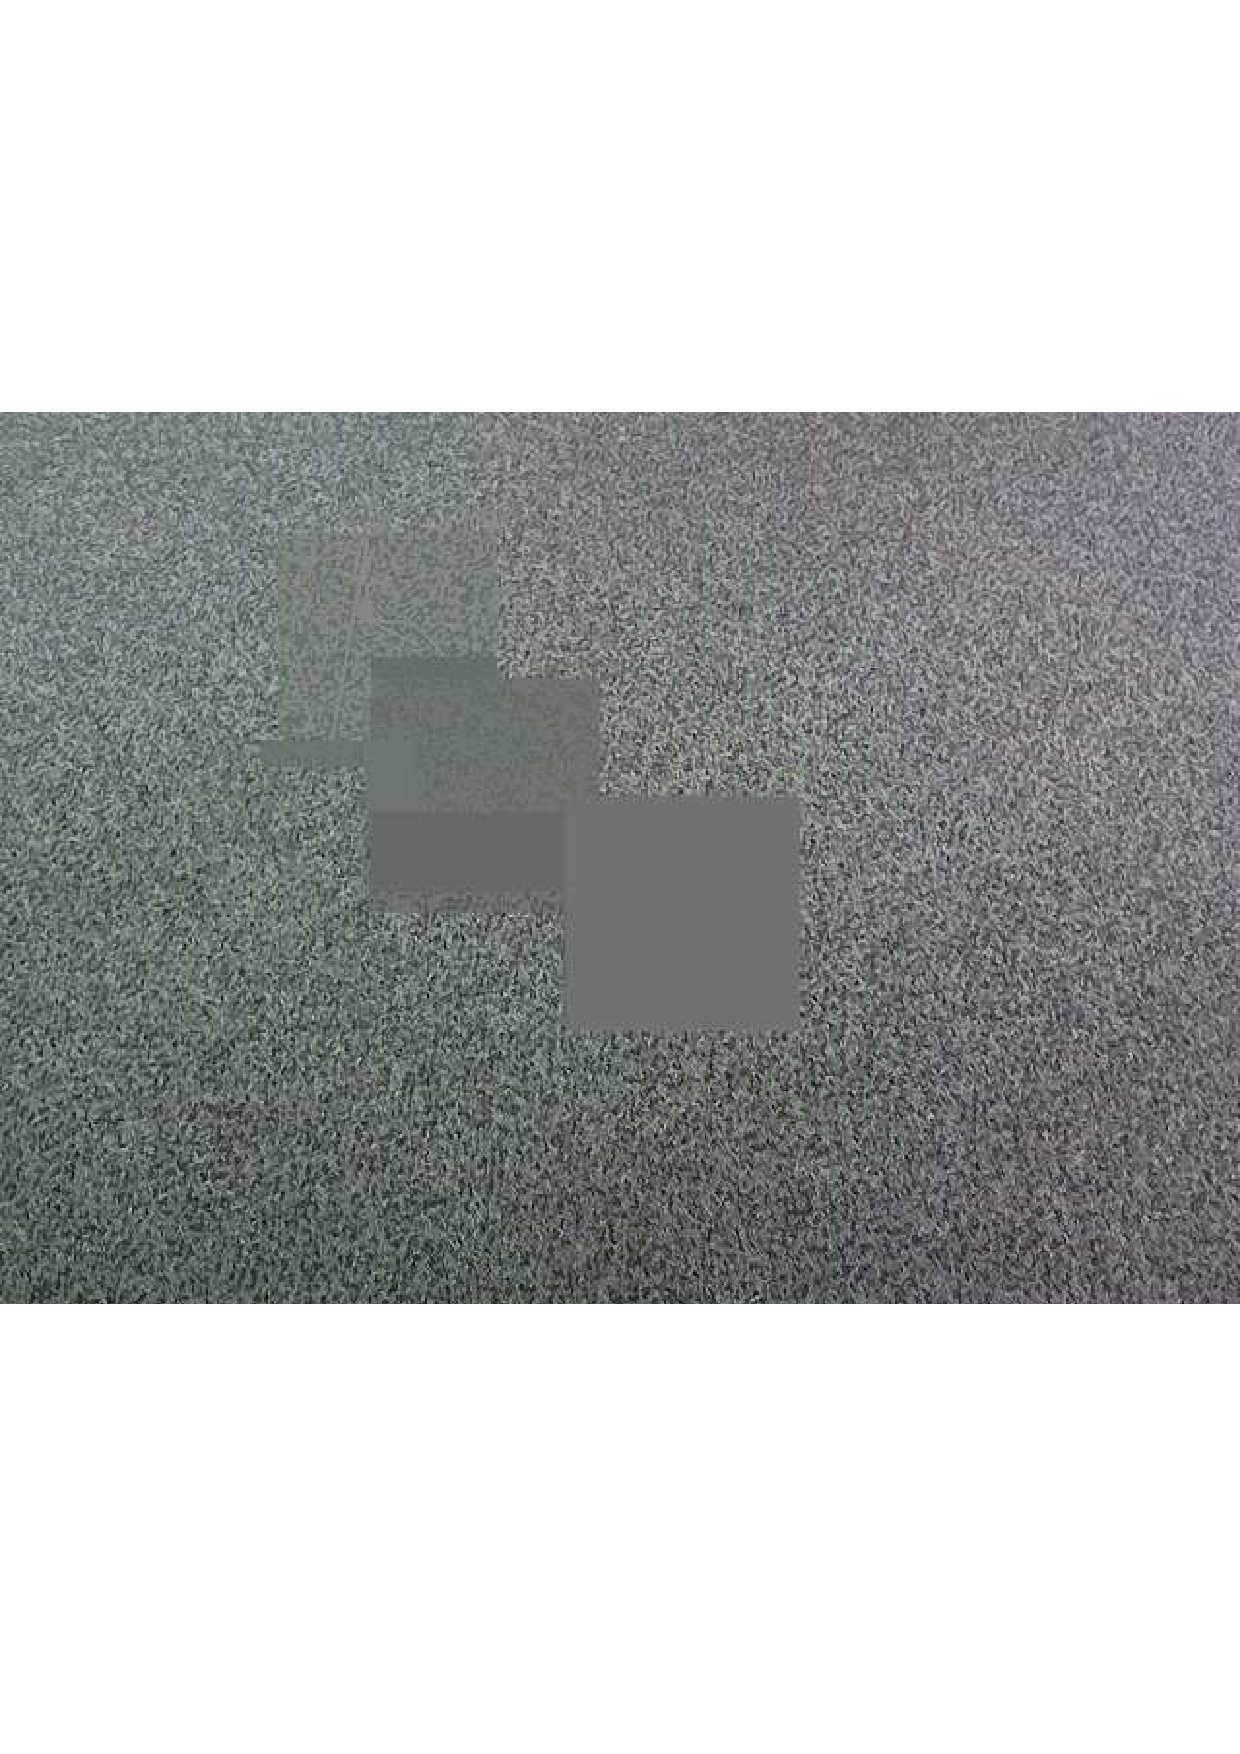
\includegraphics[scale=0.3]{../Drawings/backdata2.pdf}
\caption{The estimated background image of the second dataset provided for image processing}
\label{fig:backdata2}
\end{minipage}
\end{figure}


\begin{figure}[h!]
\begin{minipage}[b]{0.5\linewidth}
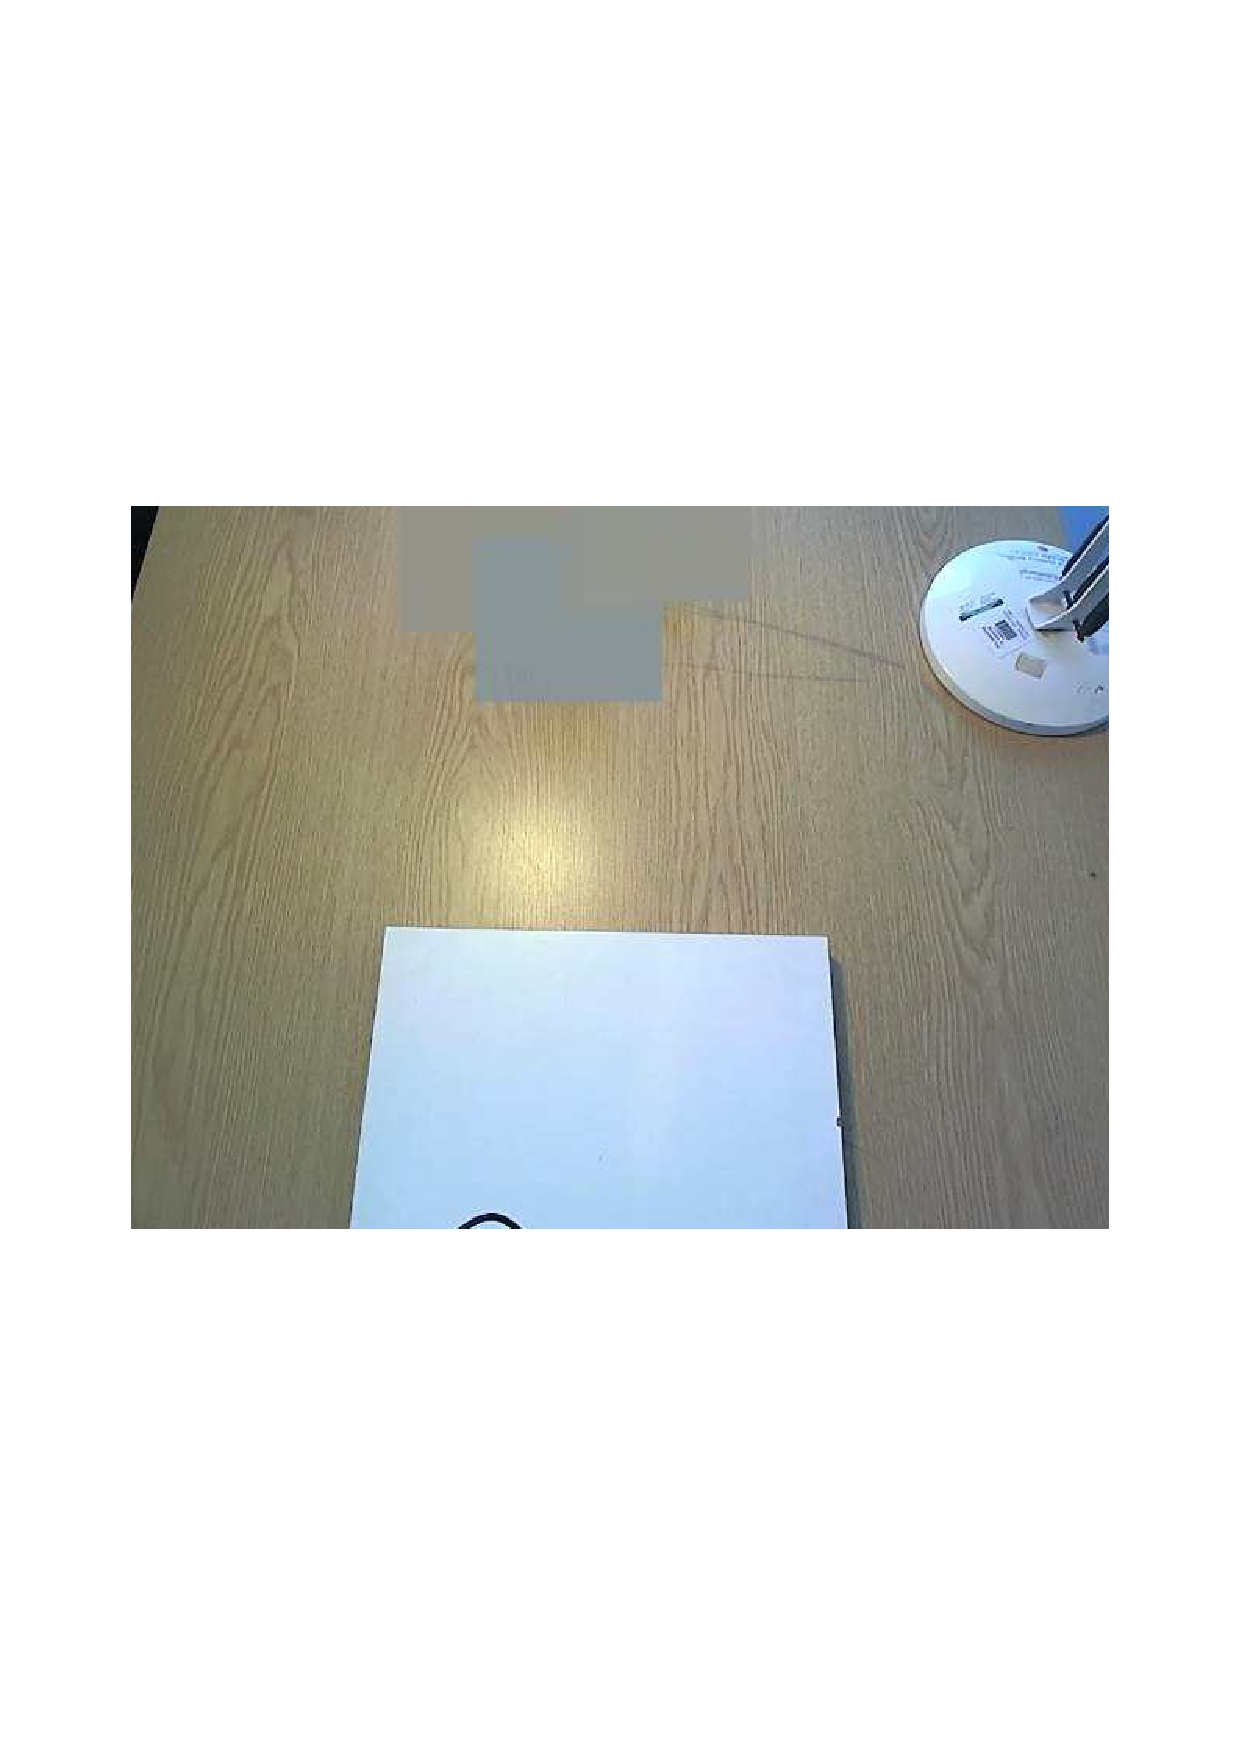
\includegraphics[scale=0.3]{../Drawings/backdata7.pdf}
\caption{The estimated background image of a new test dataset}
\label{fig:backdata7}
\end{minipage}
\hspace{0.5cm}
\begin{minipage}[b]{0.5\linewidth}
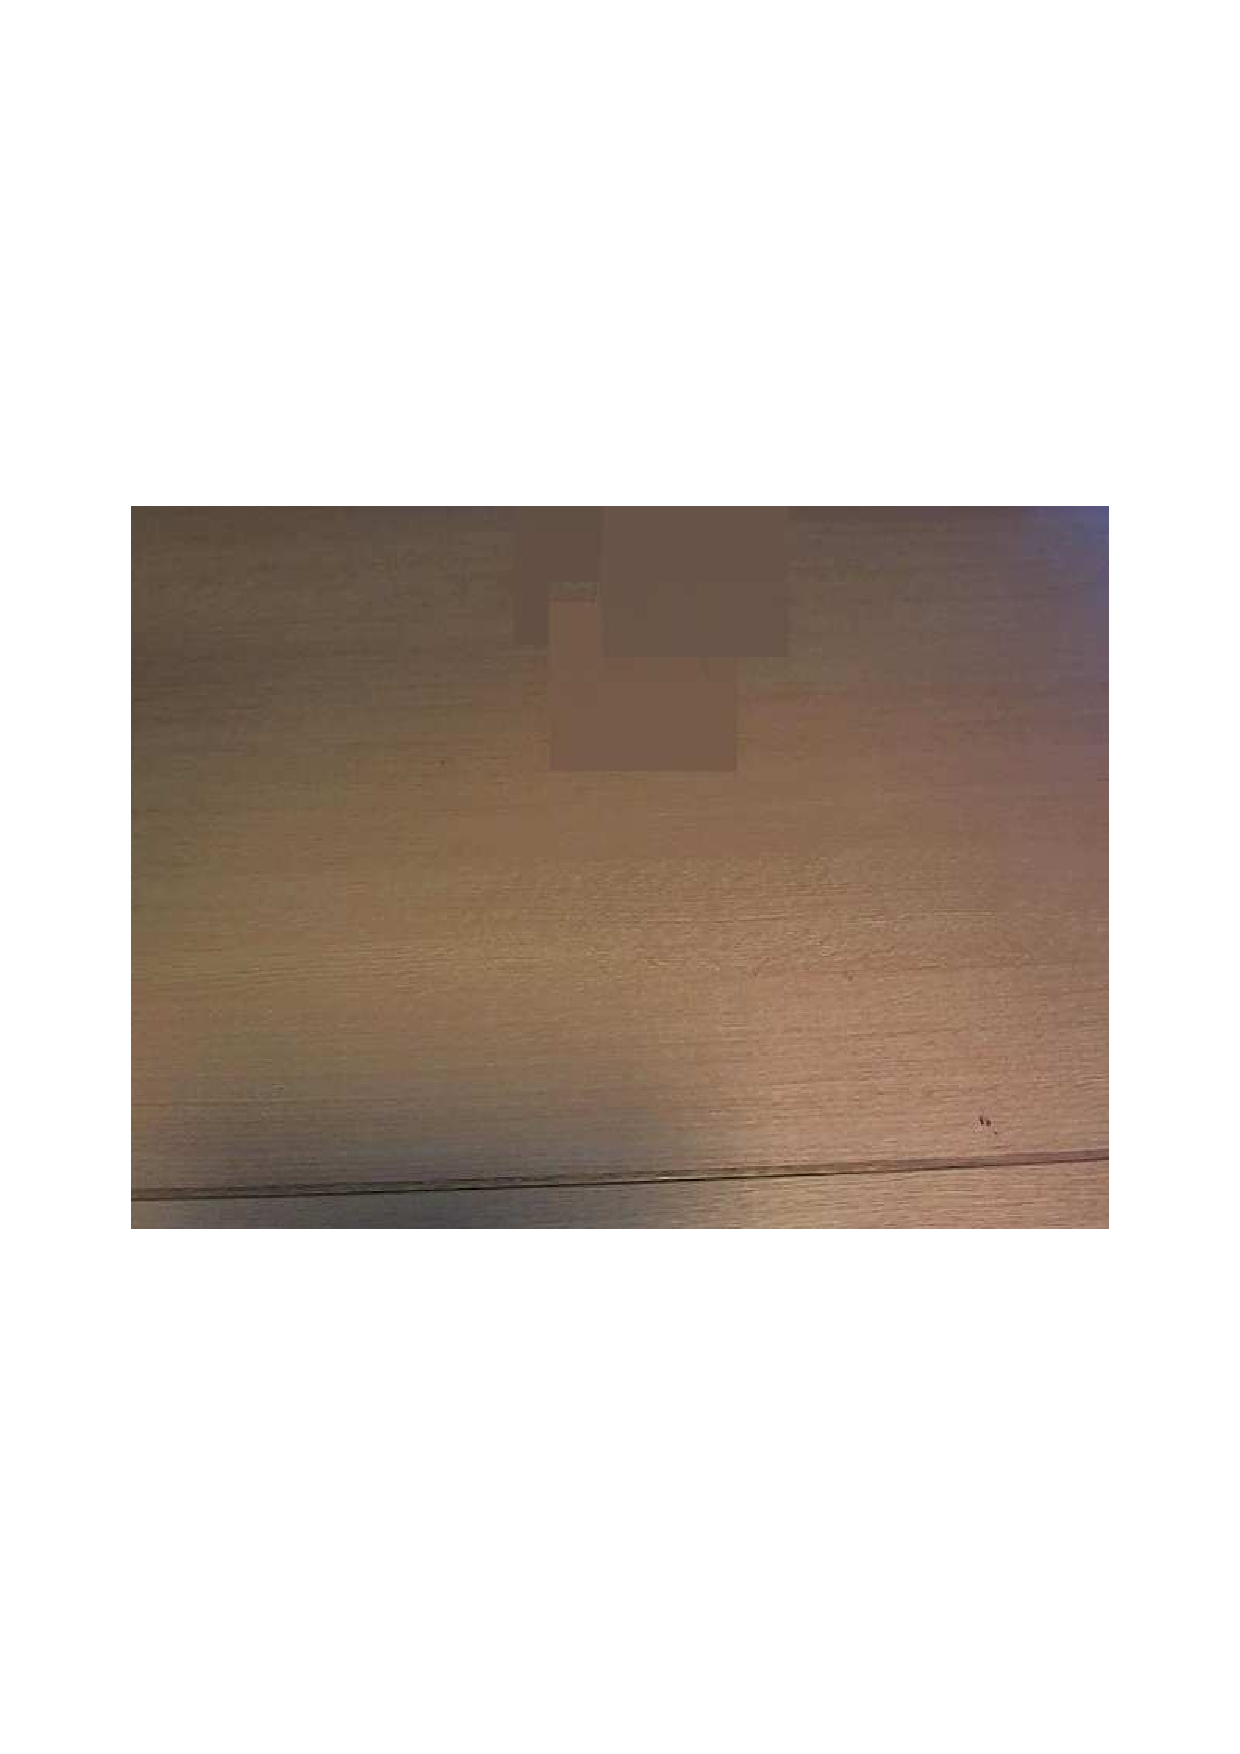
\includegraphics[scale=0.3]{../Drawings/backdata10.pdf}
\caption{The estimated background image of a new test dataset}
\label{fig:backdata10}
\end{minipage}
\end{figure}

%Show an example of results for each stage of detection

\section{Discussion}
\label{sec:discussion}
%Assess the success of the program with regard to:

%1. Report results

%Discuss any
%1. Limitations, problems
%2. Improvements you would make

\section{Code}
\label{sec:code}
%Any downloaded code should be recorded in the report. Does not need to be in the appendix
%Code from course web pages are not needed

\section{Conclusion}
\label{sec:conclusion}

%\bibliographystyle{witseie}
%\bibliography{bibliography}
 \newpage
\onecolumn
\appendix
\setcounter{table}{0}
\setcounter{figure}{0}
\setcounter{subsection}{0}
\makeatletter \renewcommand{\thefigure}{A.\@arabic\c@figure} \renewcommand{\thetable}{A.\@arabic\c@table} \renewcommand{\thesection}{A.\@arabic\c@section} \makeatother
\section*{APPENDIX A}

\section{Control Program}
%Add the matlab code to this file...
%\lstinputlisting{codeSnippets.cpp}
 
\end{document}

